\subsection{The Controller}
\label{sec:ppcontroller}
The pure-pursuit controller~\cite{Amidi.1991}
as formulated in~\cite{Snider.2009} is used to determine the steering angle.
This simple controller was ``the most stable and accurate tracker"
of the three methods tested in~\cite{Amidi.1991}.
Furthermore, pure-pursuit performed
``fairly well and is quite robust to large errors and discontinuous paths" in comparison to a few more complicated (geometric, kinematic or dynamic) controllers~\cite{Snider.2009}.

% \begin{figure}
% \centering
% 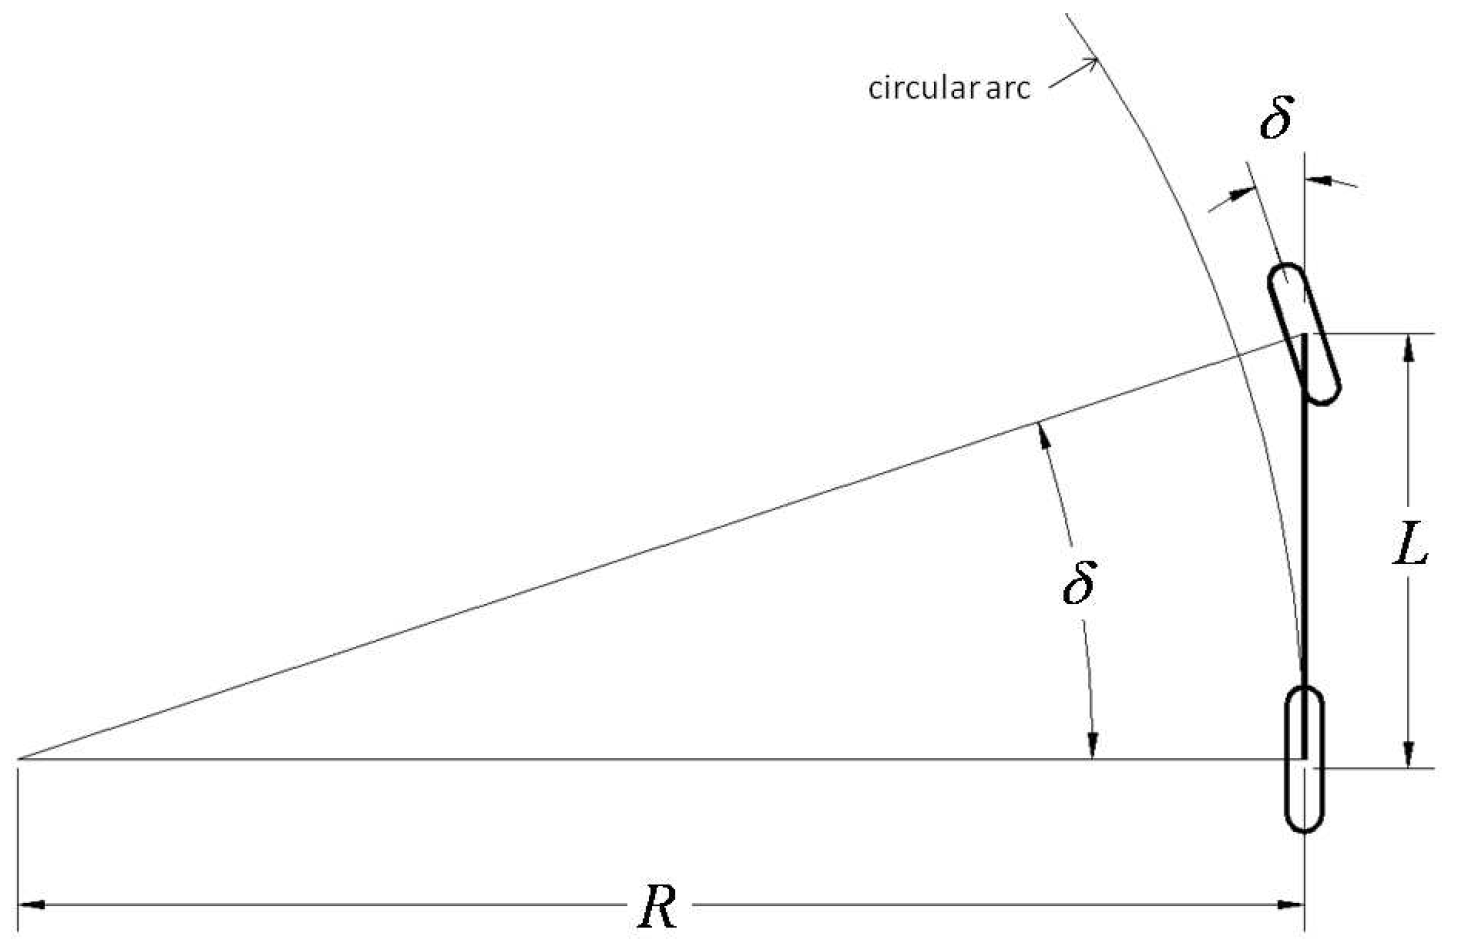
\includegraphics[width=85mm]{Figures/BicycleModel.png}%
% \caption{Bicycle model \cite{Snider.2009}}
% \label{fig:bicycle}%
% \end{figure}
% The bicycle model (Fig.~\ref{fig:bicycle}) of the vehicle  assumes that no wheel has lateral slippage.
% Therefore,
% if the steering angle is $\delta > 0$ and the wheelbase is $L$,
% then the rear wheel moves on a circle of radius $R$ where
% \begin{equation}
% R = \frac{L}{tan(\delta)}.
% \end{equation}


\begin{figure}
\centering
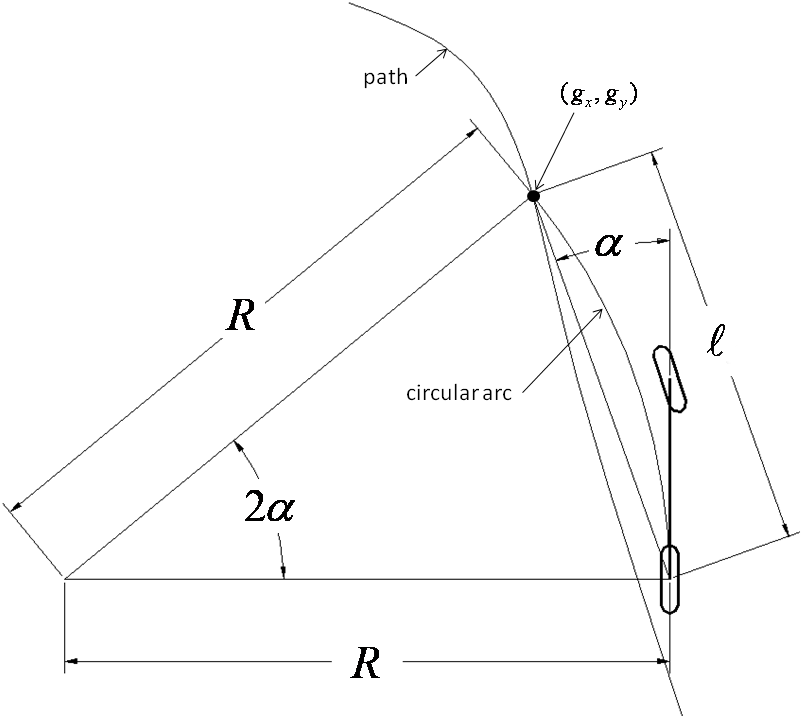
\includegraphics[width=60mm]{Figures/Purepursuit.png}%
\caption{Purepursuit controller \cite{Snider.2009}.}
\label{fig:purepursuit}%
\end{figure}

The input to the pure-pursuit controller is a waypoint described in the car's \emph{rear-axle coordinates}.
The origin of the rear axle coordinates is the center of the rear axle, the x-axis is the heading of the car, and the heading of the y-axis is 90 degrees counterclockwise from the x-axis.
The output is the steering angle $\delta$ for the bicycle model of a car.
Let $(g_x, g_y)$ be the coordinates of the waypoint in the rear-axle frame.
Note that the lookahead distance $\ell$ is $\sqrt{g_x^2+g_y^2}$.
If $L$ is the \emph{wheelbase} of the car (i.e. distance between rear and front axles), then the pure-pursuit steering angle $\delta$ is\footnote{See \cite{Snider.2009} for the derivation of the formula.}
\begin{align}
\delta & = tan^{-1}(\frac{2Lsin(\alpha)}{\ell}) \nonumber \\
 & =  tan^{-1}(\frac{2L g_y}{\ell^2})
 \label{eqn:purepursuit}
\end{align}
% \begin{center}
% \begin{equation}
% \begin{tabular}{rcl}
%     $\delta$ & $=$ & $tan^{-1}(\frac{2Lsin(\alpha)}{\ell})$ \\
%         & $=$ & $tan^{-1}(\frac{2L g_y}{\ell^2})$.
% \end{tabular}
% \label{eqn:purepursuit}
% \end{equation}
% \end{center}
Note that this formula is valid even when the waypoint is on the right of the car,
where $\alpha$, $g_y$ and $\delta$ are all negative.
This formula is valid only when $g_x > 0$
i.e. when the waypoint is on the front of the rear axle.
In this case,
we have $\frac{-\pi}{2} < \delta < \frac{\pi}{2} $.
In practice,
$-\delta_{max} \leq \delta \leq \delta_{max} $
where $\delta_{max} < \frac{\pi}{2}$ is the maximum possible angle that the car can steer.
For example,
the maximum steering angle for the Traxxas car in the open source hardware platform of F1Tenth vehicle is about $34$ degrees.

% Sridhar: Remaining part from the older control section.

% Given a plan (i.e. a piecewise linear continuous curve) from the planner,
% the controller computes the steering angle.
% The assumption of the controller is that the plan is within distance $\ell$ of the rear axle.
% Here, $\ell$ is the lookahead distance for the Pure Pursuit controller.
% Therefore, the lookahead circle (of radius $\ell$ around the rear axle) will intersect the plan,
% or the plan will be contained in the lookahead circle.
% In the former case,
% we take the intersection point that is further along the plan,
% as the Pure Pursuit goal;
% and in the latter case,
% we take the end of the plan to be the Pure Pursuit goal.

